\documentclass[letter]{scrartcl}
\usepackage{graphicx}
\usepackage{fullpage} %1in margins
\usepackage{tabularx}
\usepackage{hyperref}
\usepackage{tikz} % for diagrams
\usetikzlibrary{automata,positioning}

\newcommand{\app}{\sc{393torrent}}

\begin{document}

\title{Requirements for \app}
\subtitle{Dan Keller, Kenneth Link, Nathan McKinley, Ross Nanopoulos}
\date{} % no date

\maketitle

\begin{abstract}
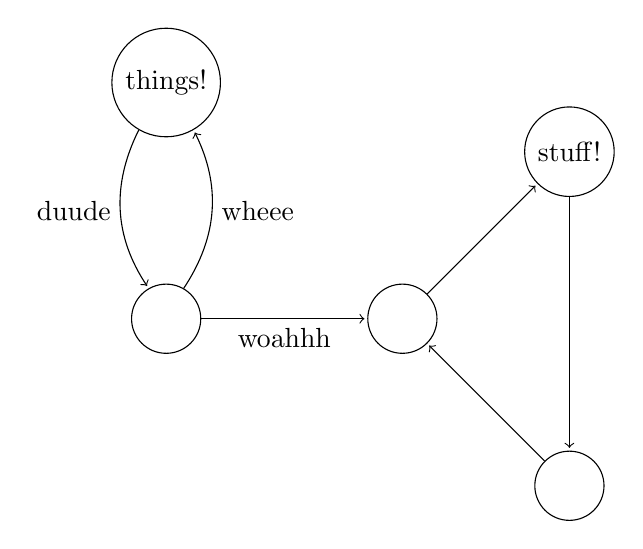
\begin{tikzpicture}[shorten >=1pt,node distance=3cm,on grid,auto]
	\node[state] (s) {};
	\node[state] (a1) [above=of s] {things!};
	\node[state] (b1) [right=of s] {};
	\node[state] (b2) [above right=of b1] {stuff!};
	\node[state] (b3) [below right=of b1] {};
	\path[->]
	(s)  edge [bend right] node [right] {wheee} (a1)
	     edge node [below] {woahhh} (b1)
	(a1) edge [bend right] node [left] {duude} (s)
	(b1) edge node {} (b2)
	(b2) edge node {} (b3)
	(b3) edge node {} (b1);
\end{tikzpicture}

The software requirements specification (SRS) specifies all user stories (i.e. functional requirements) as well as nonfunctional requirements. These requirements are used in iteration planning as well as acceptance testing.  This document should be used by the members of the 393torrent team, who will implement and verify the functionality of the BitTorrent client.
\end{abstract}

\tableofcontents
\pagebreak

\section{Overview}
The BitTorrent client (393torrent) will allow users to download, create, and seed torrent files.  It will enable them to achieve the full functionality of a BitTorrent client in a lightweight form.  The primary objective of this BitTorrent client is to offer a free and open source alternative--without advertisements--to the current heavyweight clients available.  Specific goals of 393torrent can be found in the vision and scope document.

\section{Bittorrent Protocol}

\subsection{Protocol Overview}
	
Bittorrent is a file transfer protocol created by Bram Cohen intended for sending files over unreliable networks.  A torrent is a collection of peers who are participating in the distribution of a file.  To achieve a reliable download protocol over unreliable networks, bittorrent uses many peers who send and receive small equi-sized “chunks” of data (typically 256KB).  A peer joins a torrent by registering with something called the tracker.  The tracker keeps track of all peers participating in the torrent and requires updates from each peer to continue tracking them.  The number of peers can be anything from one to thousands of peers, however the more peers the faster the download speed which is opposite of server hosted downloads.  After the tracker becomes aware of a new peer it sends that user (User A) a list of ip addresses of other peers on the torrent.  User A will attempt to connect via TCP to each of the peers obtained from the list and exchange a list of missing chunks with that peer.  With the new knowledge of which peer has the chunks that User A is missing, User A can request the rarest chunks first (a chunk that most of her peers do not have but at least one peer does have).  After the rarest first have been taken care of, User A will continue trading chunks with peers who are currently supplying User A with the highest data rate.  Also, every 10 seconds User A will recalculate the download rates and update the list of highest data rate peers.  Additionally every 30 seconds User A chooses one peer by random and sends a chunk to it. 

\subsection{Tracker}
	The tracker is a database of peers which responds to HTTP GET requests.  These requests can return tracker statistics and a list of peer ip addresses.

\begin{figure}[ht!]
\centering
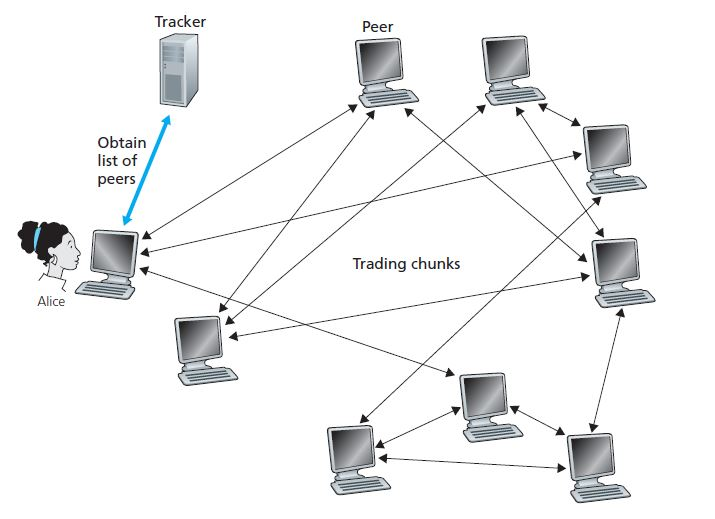
\includegraphics[width=120mm]{infographic.jpg}
\caption{Tracker infographic}
\label{overflow}
\end{figure}

Typical tracker requests may include the following parameters:
\begin{itemize}
\item info\_hash: urlencoded 20-byte SHA1 hash of the value of the info key from the Metainfo file
\item peer\_id: urlencoded 20-byte string used as a unique ID for the client, generated by the client at startup
\item port: The port number that the client is listening on
\item uploaded: The total amount uploaded (since the client sent the 'started' event to the tracker) in base ten ASCII.
\item downloaded:  The total amount downloaded (since the client sent the 'started' event to the tracker) in base ten ASCII
\item left: The number of bytes this client still has to download in base ten ASCII.
\item compact: Setting this to 1 indicates that the client accepts a compact response.
\item no\_peer\_id: Indicates that the tracker can omit peer id field in peers dictionary
\item event:  If specified, must be one of started, completed, stopped, (or empty which is the same as not being specified). If not specified, then this request is one performed at regular intervals.
\item ip: Optional. The true IP address of the client machine, in dotted quad format or rfc3513 defined hexed IPv6 address
\item numwant: Optional. Number of peers that the client would like to receive from the tracker. This value is permitted to be zero. If omitted, typically defaults to 50 peers.
\item key: Optional. An additional client identification mechanism that is not shared with any peers. It is intended to allow a client to prove their identity should their IP address change.
\item trackerid: Optional. If a previous announce contained a tracker id, it should be set here.
\end{itemize}

Trackers answer a request with a response containing a plaintext document which contains a bencoded dictionary with these keys:
\begin{itemize}
\item failure reason: If present, then no other keys may be present. The value is a human-readable error message as to why the request failed (string).
\item warning message: (new, optional) Similar to failure reason, but the response still gets processed normally. The warning message is shown just like an error.
\item interval: Interval in seconds that the client should wait between sending regular requests to the tracker
\item min interval: (optional) Minimum announce interval. If present clients must not reannounce more frequently than this.
\item tracker id: A string that the client should send back on its next announcements. If absent and a previous announce sent a tracker id, do not discard the old value; keep using it.
\item complete: number of peers with the entire file, i.e. seeders (integer)
\item incomplete: number of non-seeder peers, aka "leechers" (integer)
\item peers: (dictionary model) The value is a list of dictionaries, each with the following keys:
\item peer id: peer's self-selected ID, as described above for the tracker request (string)
\item ip: peer's IP address either IPv6 (hexed) or IPv4 (dotted quad) or DNS name (string)
\item port: peer's port number (integer)
\item peers: (binary model) Instead of using the dictionary model described above, the peers value may be a string consisting of multiples of 6 bytes. First 4 bytes are the IP address and last 2 bytes are the port number. All in network (big endian) notation.
\end{itemize}
\subsection{Peer Wire Protocol TCP}

In TCP, a client must remember state information such as:

\begin{itemize}
\item choked: When a peer uses the choke signal, it is letting the other peer’s client know that notification requests will not be answered unless the client is unchoked. 
\item interested: if the user is interested in a chunk the other peer has to offer
\item am\_choking: this client is choking the peer
\item am\_interested: this client is interested in the peer
\item peer\_choking: peer is choking this client
\item peer\_interested: peer is interested in this client
Client connections start out as "choked" and "not interested". In other words:
\item am\_choking = 1
\item am\_interested = 0
\item peer\_choking = 1
\item peer\_interested = 0
\end{itemize}

\subsection{Handshake}
The first message sent by a client is the handshake.  This is done before any connection is established between peers. 
\begin{itemize}
\item pstrlen: string length of pstr, as a single raw byte
\item pstr: string identifier of the protocol
\item reserved: eight (8) reserved bytes. All current implementations use all zeroes. Each bit in these bytes can be used to change the behavior of the protocol. An email from Bram suggests that trailing bits should be used first, so that leading bits may be used to change the meaning of trailing bits.
\item info\_hash: 20-byte SHA1 hash of the info key in the metainfo file. This is the same info\_hash that is transmitted in tracker requests.
\item peer\_id: 20-byte string used as a unique ID for the client. This is usually the same peer\_id that is transmitted in tracker requests (but not always e.g. an anonymity option in Azureus).
\end{itemize}
\subsection{Advantages}

As opposed to traditional file distribution methods, Bittorrent has fasted distribution time which increases as the number of users increases because a high number of peers means there  will be a more efficient use of bandwidth. 

\begin{figure}[ht!]
\centering
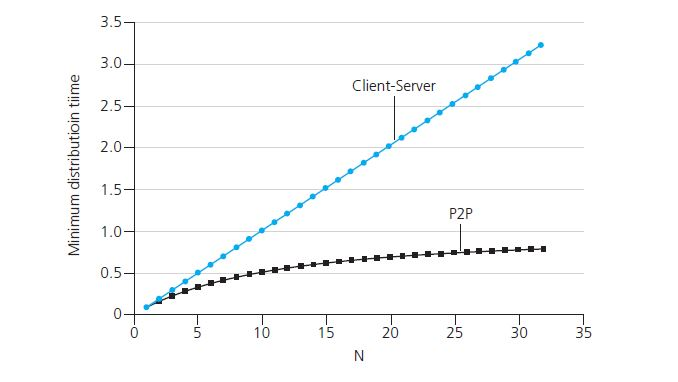
\includegraphics[width=90mm]{Graph.jpg}
\caption{Distribution time vs peers}
\label{overflow}
\end{figure}

Wiki.theory.org Contributors. (2013 July 26) `` ''Bittorrent Protocol Specification v1.0`` ''. [Online]. Available: https://wiki.theory.org/BitTorrentSpecification

Ross Kurose. `` ''Chapter 2 Application Layer`` ''. Computer Networking A Top-Down Approach 6th edition

\section{App Architecture}
A single run of this application will progress through three stages.  They are, in brief, the torrent acquisition stage, the file download stage, and the file seeding stage.  In the first stage, the application will determine what trackers it should connect to, and which files it is attempting to download.  The output of this stage will be an object containing the trackers that will be used for this torrent download, and the information about the torrent download itself.  This output is used as input to the second stage of the application run, which will proceed with the connections to peers and begin downloading individual "pieces" (as defined by the bittorrent spec) from those peers.  After several sequential pieces have been received, those will be combined into a "part", which will be saved to disk.  After all pieces have been downloaded, the parts which have been saved to disk will be combined into the output file.  In the final stage, the pieces will be served to other peers which request them.

This third stage will begin at the same time as the second stage, since pieces which have been downloaded already can be served up even before the entire file has been received.  In some sense, this is the reason that the bittorrent protocol leads to decreased time to complete a download.  It will also be continued after download is complete, if the user has specified that they would like to continue seeding indefinitely.

\begin{figure}[h]
\centering
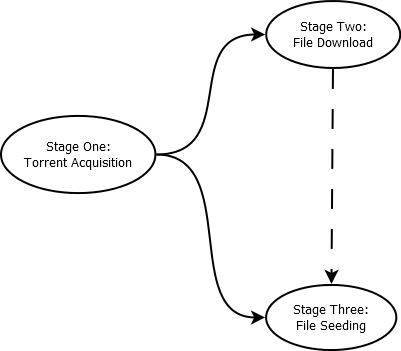
\includegraphics[scale=.5]{stageDiagram.png}
\caption{The three stages of an application run}
\end{figure}

\subsection{Torrent Acquisition Stage}

\begin{figure}[h]
\centering
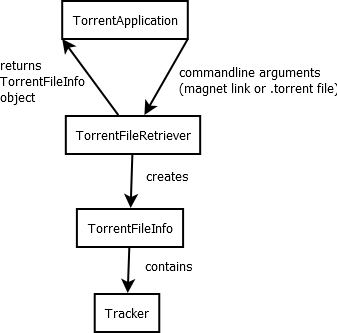
\includegraphics[scale=.5]{StepOne.png}
\caption{The four objects involved in the first stage of an application run}
\end{figure}

In this first stage of an application run, the TorrentApplication (our main class) will create a TorrentFileRetriever.  This object is responsible for understanding the command-line arguments passed to the application, whether they be a magnet link or the location of a file in the filesystem.  Since we seek to be cross-platform, we will need to defer to the OS for this kind of understanding; we'll need to understand '/home/username/something.torrent' on unix as well as as 'C:\textbackslash Documents And Settings\textbackslash Username\textbackslash something.torrent' on Windows.  This is easily possible due to python's os.path module, which understands cross-platform filenames.\\

The TorrentFileRetriever will either read or download information about the torrent that the user seeks to download, depending on input.  In either case, it will return a TorrentFileInfo object, which will contain information that the rest of the application will require in order to function.  This information includes the SHA1 hash of the 'info' dict contained in the .torrent file, as well as several other key pieces of information (announce URL, etc).  See Section One for details on the information which will need to be present.\\

Very important in this TorrentFileInfo object will be a Tracker object, which will have the capability to connect to the torrent tracker(s) specified in the .torrent file.  There are very specific messages that need to be sent to the trackers at intervals during download; the Tracker object will be capable of sending these and reading their responses.

\subsection{File Download Stage}

\begin{figure}[h]
\centering
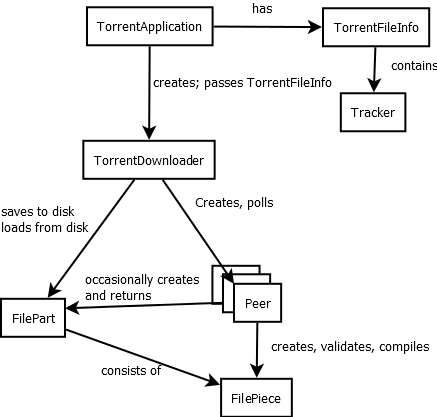
\includegraphics[scale=.5]{StepTwo.png}
\caption{The objects involved in the second stage of an application run}
\end{figure}

The second stage begins immediately after the first stage completes.   In this stage, the TorrentApplication creates a TorrentDownloader which is responsible for downloading the contents of the torrent.  The TorrentDownloader takes in a TorrentFileInfo object which has information about available trackers.  When the number of active peers falls below a preconfigured threshold (choice of this threshold has been empirically shown to affect performance, 30 is a good default), the TorrentDownloader will query the trackers for additional peers, and create Peer objects for each of these peers.  These Peer objects are responsible for handling communication with the peers, coordinated by the TorrentDownloader.  This central coordination will ensure that no file pieces are downloaded multiple times.\\

One operation available on Peer objects will be the download\_piece(int piece\_num) operation.  When a piece finishes downloading, a FilePiece object will be created.  Over time, FilePiece objects will be collected into FilePart objects (in order to reduce disk writes), which will be serialized to disk.  Once all pieces are done downloading (a condition recognized by the TorrentDownloader), the FilePart objects will be loaded, one by one, and have their contents written into the file(s) that the .torrent file specifies.

\subsection{File Seeding Stage}
\begin{figure}[h]
\centering
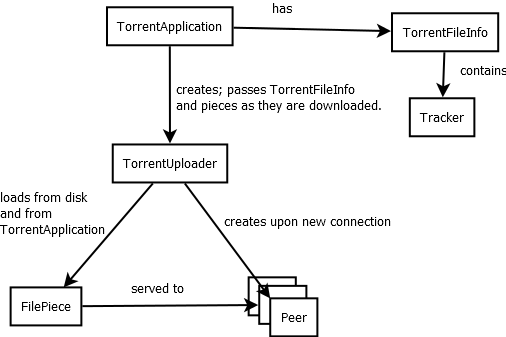
\includegraphics[scale=.5]{StepThree.png}
\caption{The objects involved in the third stage of an application run}
\end{figure}

The third stage begins immediately after the first stage completes, and may live indefinitely (until killed) if the user specifies on the command line that they wish to seed indefinitely.  In this stage, the TorrentApplication creates a TorrentUploader, which loads the state of the download from disk (by reading the FilePieces).  It then opens a port for connections from peers (by default, this port will be 6881, but this will be configurable), and waits for connections to begin.  When connections are initiated, the TorrentUploader will create new Peer objects for each connection (since peers are allowed only one connection each) and will serve requests by reading the FilePieces from disk.  This is done to reduce memory overhead; if the FilePieces were held in memory so that upload requests would not cause disk reads, we would need to hold at least the total filesize in memory.  Since torrents are often used for very large downloads (in some cases, multiple terabytes), this is infeasible.

\section{Thread Model}

\section{Classes in Detail}

\pagebreak
\section{Author Contributions}
This section provides the details to what each author contributed to the vision and scope document, as requested per professor Podgurski.
\subsection{Daniel Keller}
Created document outline and 
\subsection{Kenneth Link}
Kenneth Created the Protocol secttion
\subsection{Nathan McKinley}
Nathan McKinley created the app architecture section and diagrams.
\subsection{Ross Nanopoulos}


\section{Inspection}
\begin{tabularx}{\textwidth}{X c c}
\textbf{Comment} & \textbf{Reported By} & \textbf{Fixed By} \\
\textbf{No Issues seen} & \textbf{Kenneth Link} & \textbf{N/A} \\
\end{tabularx}
\end{document}
